\documentclass[oneside,12pt]{amsart}
\usepackage[english]{babel}
\usepackage{graphicx}
\usepackage{float}
\usepackage{mathtools}
\usepackage{amsfonts}
\usepackage{amssymb}
\usepackage{siunitx}
\usepackage{amsthm}
\usepackage{enumitem}
\usepackage{stmaryrd}
\usepackage{multirow}
\usepackage[backend=bibtex,style=numeric]{biblatex}
\bibliography{Biblio}
\usepackage[a4paper, total={6in, 10in}]{geometry}
\graphicspath{{./}{}}% You can add the path for the images in the empty brackets 
\title{Exploring Electrostatics}
\author{Michael Kulinich, Jayson Marshall, Daniel Briseno}
\date{}
\newdimen\graph
\graph=4.2in
\newdimen\medgraph
\medgraph = 5.3in
\newdimen\smallgraph
\smallgraph = 3in
\newdimen\tinygraph
\tinygraph = 1.5in
\renewcommand{\arraystretch}{1.5}

\begin{document}
	\maketitle
	\section{Abstract}
	In this experiment, we studied Gauss’ law by studying the electric field lines generated by a charged particle. We found that the density of the electric field lines at a point had a positive correlation with the strength of the electric field at that point and that the number of field lines generated by a particle is directly proportional to the magnitude of that charge.
	
	
	\section{Introduction}
	In previous labs, Coulomb’s law was calculated to find the force on a test charge due to charges within a distance $r$. Electric fields have been defined as a vector that describes the direction and magnitude of the force exerted on a positive test charge per unit charge.  It too can be calculated using Coulomb’s law, however using Gauss’s law, which involves relating the electric field surrounding a collection of charges to the net amount of charge inside a closed surface. In this lab, we will see how to present the electric field in a region of space by using electric field lines, define electric flux (quantity related to electric field lines), and attempt to rediscover Gauss’s law by drawing closed surfaces around various charges and/or groups of charges, along with seeing how many electric field lines cross in and out of the surface.
	\newpage
	\section{Procedure and Analysis}
	
	\subsection{Activity 1-1 pt.1}We set a single +1 charge on the screen as an arbitrary unit and ran the program. Next, a -1 charge was placed at another location on the screen, and the field lines associated with it are displayed in the screenshots. This process was repeated with varying charges.
		\subsubsection{Question 1-1: How many lines are there in the drawings? Are the lines more dense (closely spaced) or less dense near the charge? Explain. How do the directions of the lines depend on the sign of the charge? }
     	
     	\paragraph{}
	
		\begin{figure}[H]
		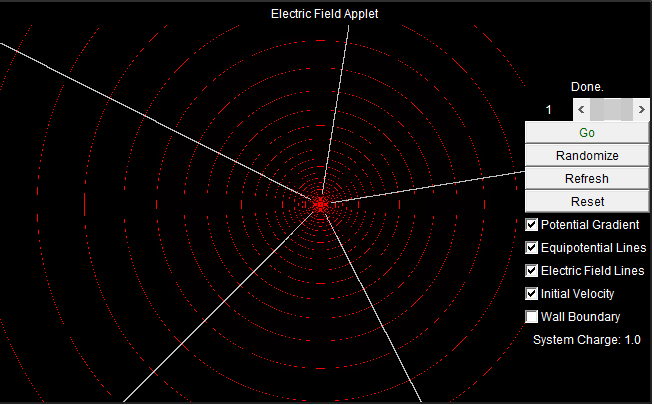
\includegraphics[width=\medgraph,scale=0.01]{Pos.png}
		%h (here) - same location
		%t (top) - top of page
		%b (bottom) - bottom of page
		%p (page) - on an extra page5
		%! (override) - will force the specified location
		\caption{Unit positive charge.} 
		\label{Pos}
	\end{figure}

	\begin{figure}[H]
	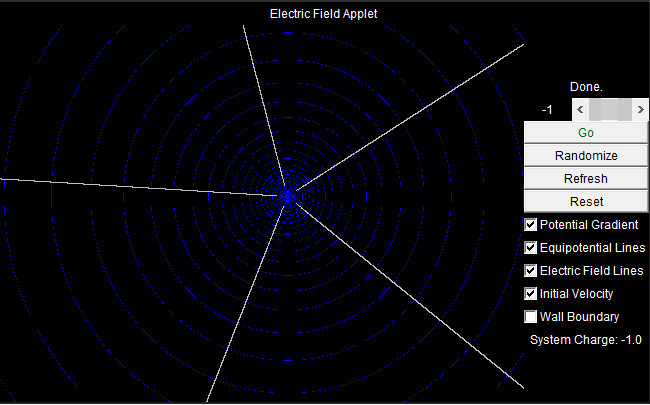
\includegraphics[width=\medgraph,scale=0.01]{Neg.png}
	%h (here) - same location
	%t (top) - top of page
	%b (bottom) - bottom of page
	%p (page) - on an extra page5
	%! (override) - will force the specified location
	\caption{Unit negative charge.} 
	\label{Neg}
	\end{figure}
There are five lines in each drawing that become more closely spaced near the charge. As the lines become more dense, the magnitude of the electric force becomes greater. In Figure \ref{Pos}, the direction of the lines point outwards from the charge. In Figure \ref{Neg}, the direction of the lines point inwards toward the charge. Since we use a positive charge in Figure \ref{Pos} and a negative charge in Figure \ref{Neg}, we can conclude that positive charges generate outward field lines and negative charges generate inward field lines.

\subsubsection{Question 1-2: What is the magnitude of your new charge? How many lines are shown in the simulation? How do the number of lines compare to the number in Question 1-1?}
\paragraph{}

\begin{figure}[H]
	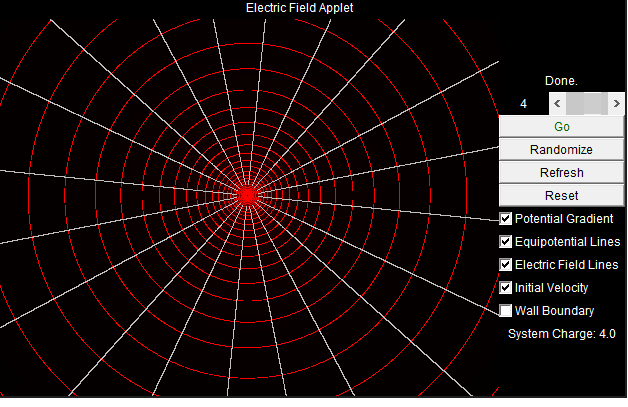
\includegraphics[width=\medgraph,scale=0.01]{BigPos.png}
	%h (here) - same location
	%t (top) - top of page
	%b (bottom) - bottom of page
	%p (page) - on an extra page5
	%! (override) - will force the specified location
	\caption{Positive charge of 4q} 
	\label{BigPos}
\end{figure}
For a charge with a magnitude of 4 units ( Figure \ref{BigPos}), there was found to be 20 field lines emanating. This is a proportional increase from Question 1-1 in which 5 lines emanated from a charge of 1 unit.


\subsubsection{ Question 1-3: If you know the magnitude of the charges, describe the rule for telling how many Ii.Iles will come out of or into a charge in this simulation. Explain your answer based on your observations.}
\paragraph{}
\indent We have empirically determined that each unit of charge generates 5 field lines, and that the direction of the field lines depends on the sign of the charge: positive charges generate field lines directed away from the source particle, negative charges generate field lines directed towards the source particle. This conclusion follows from our observations on images 1,2 and 3, since the field lines in all three images follow this criterion.
\newpage

\subsection{Activity 1-1 pt.2}We repeated the exercise using two charges of the same magnitude but opposite sign. The results are shown in Figure \ref{PosNeg}

\begin{figure}[H]
	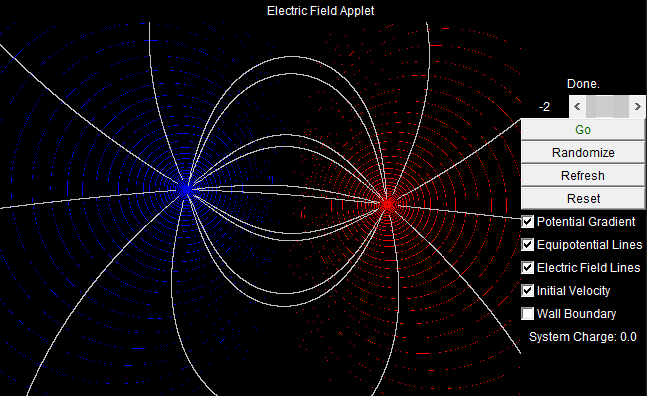
\includegraphics[width=\medgraph,scale=0.01]{PosNeg.png}
	%h (here) - same location
	%t (top) - top of page
	%b (bottom) - bottom of page
	%p (page) - on an extra page5
	%! (override) - will force the specified location
	\caption{ Two charges with +2 and -2 unit charge respectively } 
	\label{PosNeg}
\end{figure}

 
\subsubsection{ Question 1-4: Are the lines beginning or ending on a charge more dense near it or far away from it? How does the direction of the lines depend on the sign of the charge?}
\paragraph{}
\indent The lines beginning or ending on a charge are denser near it than far away. The direction of the lines points away from a positive charge, while the direction of the lines points towards a negative charge.

\subsubsection{Question 1-5: Summarize the properties of electric field lines. What does the number of lines signify? What does the direction of a line at each point in space represent? What does the density of the lines represent?
}
\paragraph{}
\indent Electric field lines show the relative magnitude of an electric field at a point in space and the charge of the particle generating the field lines. The number of field lines generated by a particle signifies the charge of the particle. In this lab, we found that every unit of charge generated 5 field lines. The direction of the field lines indicates the charge of the source particle, with field lines pointing towards negative charges and away from positive charges. Finally, the density of the lines at a certain point represents the magnitude of the electric field at that point.

\section{Test Your Understanding}
\begin{enumerate}
	\item \textbf{Describe the properties of electric field lines.}
	\begin{enumerate}
		\item \textbf{If the total number of lines leaving or converging on a charge doubles, what does that tell you about the magnitude of the charge?} \\
		\indent This tells us that the magnitude of the charge doubles since it is directly proportional to the number of lines.
		\item \textbf{What does the direction of a line at each point in space represent?}\\	
		\indent The direction of a line at each point in space represents whether a given charge is negative or positive. If the charge is negative, the lines will point in towards the charge. if the charge is positive, the lines will point out, away from the charge. 
		\item \textbf{What does the density of lines represent?}\\
		\indent As the lines become more dense, the magnitude of the electric force becomes greater.	
	\end{enumerate}
	\item \textbf{ Based on your observations of electric field lines in this lab, sketch several electric field lines originating from the +q charge. Then sketch how many lines would originate from a charge of +3q.}
	\begin{figure}[H]
		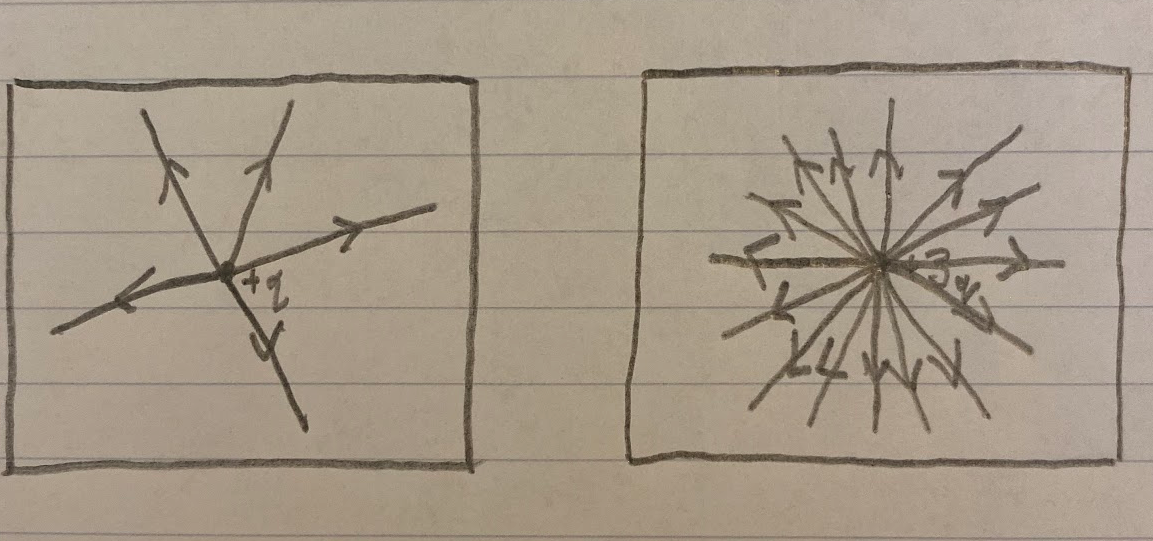
\includegraphics[width=\medgraph,scale=0.01]{Sketch.png}
		%h (here) - same location
		%t (top) - top of page
		%b (bottom) - bottom of page
		%p (page) - on an extra page5
		%! (override) - will force the specified location
		\caption{Electric field diagram of +q charge (left) and +3q charge (right)}
		\label{Sketch}
	\end{figure}
	\item We did not do Activity 1.3.
	\item \textbf{What is the net electric flux through the closed surface in each case?}
	\begin{enumerate}
		\item +1, the net flux is 5 because there’s a charge of +1 meaning 5 lines are leaving the surface
		\item 0, there’s no net charge so the net flux is 0.
		\item -1, the net flux is -5 because the charge is -1, meaning 5 lines are terminating inside the surface.
		\item 0, there’s no net charge so the net flux is 0.
	\end{enumerate}
	\item \textbf{How does Gauss’ law explain that excess charge on a conductor must reside on the outside surface?
	}\\
\indent Gauss’ law tells us that if there is any net free charge within the conductor then this also produces an electric field within the conductor. The electric field will cause the charges to move, and they will do so until this electric field is zero. Gauss's law then also tells us that this will be accomplished once there is no net free charge within the conductor, so the free charge must accumulate on the surface.

\end{enumerate}
\section{Conclusion}
In this lab, experiments were done to investigate various aspects of Gauss’ law. We also investigated how the electric field changes depending on the charge and magnitude of the object. This was investigated through simulations. 





	
	
\end{document}
